\documentclass[11pt, a4paper, twoside]{article}

% --- Packages ---

\usepackage[ngerman]{babel}
\usepackage[a4paper,top=2cm,bottom=2cm,inner=2.75cm,outer=2.75cm,marginparwidth=1.75cm]{geometry}
\usepackage{amsmath}
\usepackage{caption}
\usepackage{setspace}
\usepackage{float}
\usepackage{acronym}
\usepackage{makecell}
\usepackage{tikz}
\usepackage{xcolor}
\usepackage{tcolorbox}
\usepackage{parskip}
\usepackage{pdfpages}
\usepackage{longtable}
\usepackage{array}
\usepackage{booktabs}
\usepackage[backend=biber, style=numeric]{biblatex}
\usepackage{hyperref}
\usepackage{fancyhdr}
\usepackage{listings}
\usepackage[utf8]{inputenc}
\usepackage[T1]{fontenc}
\usepackage{color}
\usepackage{graphicx}

% --- Fonts ---

\renewcommand{\rmdefault}{ptm}  % Times New Roman
\renewcommand{\sfdefault}{phv}  % Helvetica

% --- Code Listing Style ---

\definecolor{codegreen}{rgb}{0,0.6,0}
\definecolor{codegray}{rgb}{0.5,0.5,0.5}
\definecolor{codepurple}{rgb}{0.58,0,0.82}
\definecolor{backcolour}{rgb}{0.95,0.95,0.92}

\lstdefinestyle{mystyle}{
    backgroundcolor=\color{backcolour},
    commentstyle=\color{codegreen},
    keywordstyle=\color{magenta},
    numberstyle=\tiny\color{codegray},
    stringstyle=\color{codepurple},
    basicstyle=\ttfamily\footnotesize,
    breakatwhitespace=false,
    breaklines=true,
    captionpos=b,
    keepspaces=true,
    numbers=left,
    numbersep=5pt,
    showspaces=false,
    showstringspaces=false,
    showtabs=false,
    tabsize=2,
    language=Python
}

\lstset{
    style=mystyle,
    literate=
        {Ö}{{\"O}}1 {Ä}{{\"A}}1 {Ü}{{\"U}}1 {ß}{{\ss}}1
        {ü}{{\"u}}1 {ä}{{\"a}}1 {ö}{{\"o}}1 {~}{{\textasciitilde}}1
}

\addbibresource{literatur.bib}

% --- Header and Footer ---

\pagestyle{fancy}
\fancyhf{ }
\lhead{Hochschule Düsseldorf}
\cfoot{\thepage}
\rhead{878007}
\fancyhead[LE]{Hochschule Düsseldorf}
\fancyhead[RO]{878007}
\fancyhead[LO]{Hochschule Düsseldorf}
\fancyhead[RE]{878007}
\renewcommand{\headrulewidth}{0.5pt}
\renewcommand{\footrulewidth}{0.5pt}
\raggedbottom

% --- Document Start ---

\begin{document}

% --- Title Page ---

\pagestyle{empty}
\begin{titlepage}
    \thispagestyle{empty}

    % Bilder links und rechts ausrichten, etwas mehr Abstand nach außen und oben
    \vspace*{1cm} % Abstand von der oberen Kante
    \begin{minipage}{0.45\textwidth}
        \raggedright
        
\includegraphics[width=0.7\textwidth]{Graphics/HSDLogo} % Etwas größere Breite
    \end{minipage}%
    \hfill
    \begin{minipage}{0.45\textwidth}
        \raggedleft
        
\includegraphics[width=0.7\textwidth]{Graphics/FacultyOfMedia} % Etwas größere Breite
    \end{minipage}

    \vspace{1.5cm} % Abstand nach den Logos

    \center

    \textsc{\Large wissenschaftliche Vertiefung}\\[2cm]

    \huge{Der Fortschritt}\\[0.2cm]
    \huge{automatischer Musiktranskriptionssysteme}\\[0.2cm]
    \huge{durch künstliche Intelligenz}\\[2cm]
    \Large

    % Informationen untereinander zentrieren
    \begin{center}
        \textit{Autor:} \\
        Benedikt Kolodziej \\
        878007 \\
        Medieninformatik (B. Sc.) \\[1cm]

        \textit{Betreuender Professor:} \\
        Prof. Dr. Dennis Müller\\
        dennis.mueller@hs-duesseldorf.de \\[1cm]

        \textit{Zeitraum} \\
        28.05.2025 - xy
    \end{center}

    \vspace{3cm} % Weniger Abstand vor dem Unterschriftenbereich

    %\begin{flushleft}
    %    Unterschrift Praxisstellenbetreuung
    %    \vspace{0.5in}

    %    \rule{0.3\textwidth}{0.4pt} \hspace{1cm} \rule{0.3\textwidth}{0.4pt}\\
    %    \makebox[0.3\textwidth][l]{Ort, Datum} \hspace{1cm} \makebox[0.3\textwidth][l]{Unterschrift}
    %\end{flushleft}
\end{titlepage}



\newpage

% --- Table of Contents and Lists ---

\setcounter{tocdepth}{3}
\tableofcontents
\newpage

\listoffigures
\newpage

% --- Main Content ---

\pagestyle{fancy}
\setcounter{page}{1}
\pagenumbering{arabic}

\section{Einleitung}
Hier kommt deine Einleitung hin. Du kannst diese Datei einfach weiter schreiben.

\section{Geschichtliche Entwickelung von AMT-Systemen}

\subsection{Moorer und eines der ersten Musiktranskriptionssysteme}
\subsubsection{Grundlegende Probleme bei AMTs}
Einer der ersten Papers über Automatic Music Transcription wurde von James A. Moorer im Jahr 1977 geschrieben.
\cite{Moorer1977}
In diesem beschreibt Moorer seinen Ansatz, polyphone Musik Audiospuren
direkt über Computerprogramme in Notenschrift zu übertragen.
Während dieses Prozesses fallen ihm schon sehr viele schwierigkeiten auf, die auch in späteren Papern und Arbeiten
eine ausschlaggebende Rolle spielen werden.

Eines dieser Probleme wird von ihm als das \("\)Cocktail-Party-Problem\("\) bezeichnet.
Dieses stellt die Schwierigkeit dar, auf einer Party bestimmten Stimmen zu folgen, während viele verschiedene Stimmen
gleichzeitig erklingen.
Das gleiche Problem liegt in der Noten transkription.
Die meisten Musikstücke haben mehrere Instrumente, welche gleichzeitig spielen.
Öfter gibt es auch Musikstücke wo es für ein Instrument, wie zum Beispiel Violine, mehrere verschiedene Stimmen gibt.
Dies erschwert die Zuordnung bestimmter Noten zu einer gewählten Stimme.
Schon viele Menschen scheitern deshalb daran große Musikstücke richtig zu transkribieren.
Noch schwieriger wird es hier für Computerprogramme.
Anfangs identifizieren diese bestimmte Töne anhand der Frequenz des Tons.
Leider reicht das, wie Moorer feststellt, nicht aus um genaustens zu bestimmen,
welche Töne genau momentan gespielt werden.

Jeder Ton hat Obertöne.
Diese Obertöne sind jeweils das Vielfache von dem Grundton, den man spielt.
Heißt, wenn ich auf einem Klavier den Ton C3 mit 130,81 Hz spiele dann hat dieser
die Obertöne C4 (261,62 Hz), G4 (392,42 Hz) usw.
Wenn man nur C3 spielt erklingen für das Computerprogramm auch die jeweiligen Obertöne,
was man Frequenzüberlagerung nennt.
Diese Frequenzüberlagerung sorgt dafür, das zum Beispiel ein Klavier anders klingt als eine Violine.
Daraus resultiert dann die Klangfarbe (Timbre) eines bestimmten Instrumentes.
\cite{goswami2013timbre}
Leider konnte Moorer zu dieser Zeit noch nicht die Klangfarbe eines Instruments erkennen.
Er konnte auch noch nicht das Problem der Obertöne lösen,
da die damaligen Algorithmen und Verfahren noch nicht in der Lage waren die Grundfrequenz von den Obertönen zu trennen,
weshalb er sich ausschließlich auf zweistimmige polyphone Musikstücke fokussierte.

Ein weiteres Problem war Rauschen in realistischen Audiospuren und
Stilistische mittel in der Musik, wie zum Beispiel Vibrato.
In real aufgenommenen Audiospuren gibt es immer ein gewisses Hintergrundrauschen.
\cite{iZotope2025noisefloor}
Dieses kann von einem Computerprogramm auch als Note erkannt werden oder verhindern, das bestimmte Noten
richtig vom Computerprogramm erkannt werden.
Moorer hat ein Musikstück analog aufgenommen und dieses dann mit einem 14-Bit converter digitalisiert.
Dadurch war das Rauschen nicht weg, aber da er das Musikstück selber aufgenommen hat und dieses konvertiert hat
sorgte es für insgesamt geringeres Rauschen.
Zudem konnte er so die Musiker davon abhalten bestimmte Stilistische mittel zu verwenden,
um bessere Daten zur Transkription zu erhalten.
Stilistische mittel, wie Vibrato, konnten nicht genutzt werden,
da diese eine kleine aber kontinuierliche Veränderung der Frequenz verursachen.
Dadurch kann das Computerprogramm nicht korrekt erkennen, das eigentlich eine einzelne Note gespielt wurde.
Somit war der Onset und Offset der Note komplett falsch.

Das letzte Problem, was Moorer angesprochen hat, ist das Nutzen von nicht
harmonischen Instrumenten wie Trommeln oder einem Schlagzeug.
Diese Instrumente haben keinen eindeutigen Pitch für deren Töne,
sie sind eher abhängig von Rhythms und Lautstärke.
Da Moorers AMT sich jedoch auf das Frequenzmuster der Noten fokussiert,
können diese Musikinstrumente nicht berücksichtigt werden.

\subsubsection{Der Aufbau von Moorers AMT-Systems}
Moorers automatische Musiktranskriptionssystem war eins der ersten seiner Art.
Viele weiteren AMT-System leiten sich von diesen ab.

Zunächst wird ein analoges Musiksignal mit einem 14-Bit converter digitalisiert.
Dieses digitale Musiksignal wurden dann genutzt um mithilfe von Bandpassfiltern,
ein Filter welcher nur bestimmte Frequenzen durchlässt,
bestimmte Frequenzbereiche zu isolieren.
Dadurch konnte Moorer die gespielte Note und deren Dauer,
also zugleich auch deren Onset und Offset, feststellen.

Nun mussten die bestimmten Noten einer gewählten Stimme zugeordnet werden.
Dies wurde durch melodische Gruppierung verwirklicht.
Zunächst wurden Inseln gebildet.
Inseln sind Noten die sich Zeitlich vollständig überlappen.
Wir gehen davon aus das jede Stimme nur eine Note gleichzeitig spielt,
wodurch diese Noten nicht der gleichen Stimme zugeordnet werden können.
Als Nächstes müssen die anderen Noten auf verschiedene Kombinationen getestet werden.
Desto kleiner die Frequenz sprünge je Note sind, desto wahrscheinlicher gehören sie einer Stimme zu.
Zudem werden Gruppierungen von Noten erstellt, welche am wahrscheinlichsten harmonisch nacheinander gespielt worden.

Zum Schluss ließ Moorer die gewonnenen Daten durch ein Programm laufen, 
um diese dann mithilfe eines Plotters in eine Notenschrift umzuwandeln.

\subsubsection{Hidden Markov Models}
Hidden Markov Modelle (HMM) sind statische Modelle, welche sich sehr gut zur Analyse von Musikstücken eignen.
Sie wurden erstmal in den 1960er Jahren erfunden
\cite{baum1970maximization}
und sind ein zentraler bestandteil früherer AMT-Systeme.
HMMs beschreiben eine Abfolge von \("\)versteckten Zuständen\("\),
welche im Kontext von AMT-Systemen Noten im Audiosignal darstellen.
Durch indirekt beobachtbare Daten, wie zum Beispiel die Spektraldaten des Audiosignals,
können diese Noten erschlossen werden.

HMMs bestehen aus:
\begin{itemize}
    \item Zustände (States)
    \item Übergangswahrscheinlichkeiten (Transition Probabilities)
    \item Emissionswahrscheinlichkeiten (Emission Probabilities)
    \item Beobachtungen (Observations)
\end{itemize}
Nehmen wir das Beispiel eines Klaviers.
Ein Klavier hat 88 Tasten, und somit mindestens 88 Zustände.
Durch Akkorde können zudem mehr Zustände generiert werden.
Die Übergangswahrscheinlichkeit stellt dar,
wie wahrscheinliche es ist von einem Zustand zu einem bestimmten anderen Zustand zu wechseln.
Zum Beispiel könnte es wahrscheinlicher sein, dass auf die Note C4 der Ton G3 folgt statt D1,
da diese Tonfolge harmonischer und musikalisch plausibler klingt.
Dies ist jedoch nur eine Annahme anhand von gesammelten Testdaten, weshalb es nicht als Begründung ausreicht.
Deshalb kommt als zweite Instanz die Emissionswahrscheinlichkeit hinzu.
Diese gibt an, wie Wahrscheinlich ein bestimmter Zustand in der momentanen Beobachtung ist.
Die Beobachtung wird dabei zusammengesetzt aus Eigenschaften, wie Frequenzverteilung, Spektrogramm
oder anderen Merkmalen die man aus anderen Modulen herleiten kann.
Aus den gesammelten Daten kann nun mithilfe von zum Beispiel dem Viterbi-Algorithmus
% Quelle
die wahrscheinlichste Abfolge von Zuständen berechnet werden.

\subsection{MIDI-Dateien}
Notenschrift als Input für ein Computerprogramm, Synthesizer oder ähnliches ist unhandlich.
Zunächst müsste man die gespielten Noten immer wieder zu Notenschrift konvertieren
und danach diese auch noch in anderen Programmen analysieren, was sehr aufwändig werden würde.
Eine bessere lösung dafür wäre eine Datenschreibweise,
bei der alle wichtigen Informationen bestimmter Noten übersichtlich aufgeschrieben sind.
MIDI-Dateien sind dafür perfekt geeignet.

MIDI ist ein Standartprotokoll zur kommunikation zwischen
elektronischen Musikinstrumenten, Computern und anderen Geräten wie zum Beispiel Synthesizer.
Dieses Protokoll wurde 1983 erstmals eingeführt und wurde schnell zu einem Standard in der digitalen Musikindustrie.
\cite{smith1983midi}
In MIDI-Dateien werden Daten von Tönen gelagert,
welche zum Beispiel zuvor von einem elektronischen Instrument gespielt wurden oder durch AMTs erfasst wurden.

In MIDI-Dateien werden folgenden Daten gespeichert:
\begin{enumerate}
    \item \textbf{MIDI Header-Chunk (MThd):} Enthält grundlegende Informationen zur Struktur der Datei:
    \begin{itemize}
        \item Formattyp (0 = eine Spur, 1 = mehrere synchrone Spuren, 2 = unabhängige Spuren)
        \item Anzahl der folgenden MTrk-Blöcke (Tracks)
        \item Zeitauflösung (Ticks pro Viertelnote)
    \end{itemize}

    \item \textbf{MIDI Track-Chunks (MTrk):} Jede Spur enthält eine zeitlich sortierte Liste von MIDI-Events:
    \begin{itemize}
        \item \textbf{MIDI-Events:}
        \begin{itemize}
            \item Note Onset / Offset
            \item Control Change (Lautstärke)
            \item Program Change (gibt das spielende Instrument an)
            \item Pitch Bend (verändert die Tonhöhe)
            \item Aftertouch / Polyphonic Key Pressure (Druckstärke pro Taste)
        \end{itemize}
        \item \textbf{Meta-Events:}
        \begin{itemize}
            \item Set Tempo (Tempo in Mikrosekunden pro Viertelnote)
            \item Time Signature (Taktart zum Beispiel 4/4 oder 3/4)
            \item Key Signature (Tonart zum Beispiel C-Dur oder A-Moll)
            \item Track Name
            \item Lyrics
            \item Markers
            \item End of Track (Ende einer Spur)
        \end{itemize}
        \item \textbf{System Exclusive Events (SysEx):}
        \begin{itemize}
            \item Herstellerspezifische Daten wie Synthesizer-Presets oder Spezialbefehle
        \end{itemize}
    \end{itemize}

    \item \textbf{Delta-Time:} Gibt die Zeit (in Ticks) an, die seit dem letzten Event vergangen ist:
    \begin{itemize}
        \item Ermöglicht die genaue zeitliche Positionierung jedes MIDI-Events
        \item Grundlage für das Timing und die rhythmische Struktur der Datei
    \end{itemize}
\end{enumerate}
Am wichtigsten sind dabei die MTrk-Blöcke, in denen die Daten der einzelnen Noten gespeichert werden.
Dabei stellt ein Track die Eventliste einer ganzen Stimme dar,
wie zum Beispiel die Melodiestimme, eine Violine, die Pedalsteuerung eines Klaviers oder Metadaten.
Es fällt auf das diese vier Beispiele alle sehr unterschiedliche Aufgaben und bedeutungen haben.
Das liegt daran, dass in MIDI-Dateien eher zusammenhängende Funktionen gespeichert werden und nicht nur Musiknoten.

MIDI-Dateien kamen auch der Forschung für AMT-Systemen sehr gelegen,
da man nun ein standardisiertes output Format für diese Programme besaß.
Später werden diese zudem sehr Essenziell bei dem Training KI basierter AMT-Systeme.
\cite{telila2025cnn}

\subsection{Polyphone AMT-Systeme und neue Ansätze}
\subsubsection{Blackboard-System}
Moorer stellte, mit seinem AMT-System, viele grundlegende Bausteine für dieses Forschungsgebiet.
Jedoch gab es noch viele offene Probleme, die noch überwunden werden mussten.
Eines der ausschlaggebendsten Probleme stellte sich Keith D. Martin.
\cite{Martin1996}
Zuvor wurden höchstens zwei verschiedene Stimmen gleichzeitig zur Musik transkription verwendet.
Ein großer Teil von Musikstücken verwendet jedoch mehr Stimmen.
Um diese polyphonen Musikstücke zu transkribieren,
baute Martin einen neuen Ansatz eines AMT-Systems mit innovativen Modulen und Ansätzen.

Nachdem das Input Audiosignal in ein Correlogram verarbeitet wurde,
spaltet sich Martins AMT-System auf, in einen Analysepfad und einen Rhythmuspfad.
Dabei konzentriert sich der Analysepfad auf die Zusammenhänge der verschiedenen Noten,
während der Rhythmuspfad sich mehr mit der Lautstärke und den Notenanschlägen beschäftigt.
Am Ende werden diese Kenntnisse zusammengeführt.
Der Output besteht aus dem Onset, der Dauer und der Frequenz jeder gespielten Note.
Martin gibt nicht explizit zurück, welcher Stimme jede Note zugeordnet ist.
Durch das Blackboard-System, und vor allem nach sequentieller Analyse der Intervalle, kann man
jedoch die erhaltenen Noten später bestimmten Stimmen nachträglich korrekt zuordnen.

\begin{figure}[H]
    \centering
    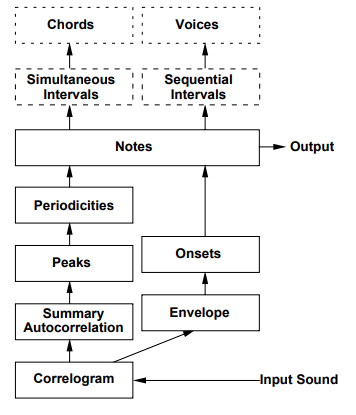
\includegraphics[width=0.6\textwidth]{Graphics/Martin1996Structure}
    \caption{Systemstruktur des AMT-Ansatzes von Keith D. Martin (1996), basierend auf \cite{Martin1996}.}
    \label{fig:martin-structure}
\end{figure}

Martin nutzte ein Blackboard-System zur Notenerkennung und Hypothesenbildung.
Unter anderem kann man dadurch Noten bestimmten Stimmen zuordnen.
Ein Blackboard-System ist ein kollaboratives Problemlösungsmodell, welches aus verschiedenen Modulen besteht,
die alle auf einem gemeinsamen Datenraum Hypothesen aufstellen können.
Um diese Vermutungen aufstellen zu können müssen jedoch erst die dafür nötigen Daten erarbeitet werden.
Dies erreicht Martin mithilfe von Sinuskurvenanalyse.
Zur Sinuskurvenanalyse, in Martins Aufbau, gehören die Bestandteile
Correlogram, Envelope, Summary Autocorrelation und Peaks.
Durch diese können Eigenschaften der Noten ermittelt werden, auf denen aufbauend später Hypothesen entstehen.
Die Module des Blackboard-Systems sind dementsprechend
Onsets, Periodicities und Simultaneous, Sequential Intervals.
Diese Module geben sich gegenseitig mehr Informationen über die gespielten Noten,
sodass später gegebene Stimmen unterschieden werden können.

Der Analysepfad beginnt bei dem Correlogram.
Hier wird der Input, ein reales Audiosignal,
zunächst verarbeitet und dann in einem Correlogram dargestellt.
Dieses Visualisiert die Korrelation der gegebenen Noten in Abhängigkeit der Zeit, Frequenz und Lag.
Lag soll in diesem Fall darstellen, wann sich ein bestimmtes Signal wiederholt.
Dabei ist die Wiederholung ein Signal, welches dem Ursprungssignal maximal selbst ähnelt.
Heißt, wenn ich einen Ton mit der Frequenz x spiele
und dieser sich nach zum Beispiel 10ms wiederholt wird das rechnerisch durch den Lag dargestellt.
Als Nächstes wird mithilfe der Summary Autocorrelation das Correlogram komprimiert
und die Datenstruktur normalisiert.
Dadurch entsteht eine stabile Grundfrequenz,
sodass die weiteren schritte effizient das Correlogram untersuchen können.
Nun werden basierend auf der normierten Struktur die Peaks gesucht.
Diese Peaks deuten darauf hin, wann periodische Komponenten auftreten.
Dabei geben sie nicht den Onset der Noten zurück, sondern nur die generelle Frequenz zu einer bestimmten Zeit.
Darauf werden mehrere Peaks, die regelmäßig wiederkehren, gruppiert.
So kann man Muster in der gespielten Musik erkennen und kurzzeitige Störfaktoren ausschließen.

Im Rhythmuspfad wird wiederum die zeitliche Analyse der Noten durchgeführt.
Zunächst wird mit dem Envelope die Lautstärke des Signals zu jedem Zeitpunkt festgelegt.
Dies dient als Grundlage, um anschließend die Onsets der Noten zu bestimmen.
Jeder Onset wird sehr präzise im Envelope dargestellt durch einen plötzlichen Anstieg der Lautstärke.

Nachdem die beiden Pfade durchgelaufen sind, hat man schon Noten,
welche man grundsätzlich in Notenschrift transkribieren kann.
Jedoch sind diese Noten musikalisch noch nicht verstanden worden.
In der oben gegebenen Abbildung gibt es noch die Bestandteile Simultaneous und Sequential Intervals.
In dem Modul Simultaneous Intervals wird ermittelt, welche Töne gleichzeitig erklingen.
Diese können, wenn sie harmonisch zueinander sind, zu einem Chord gebunden werden.
Sequential Intervals analysieren dahingegen, welche Töne nacheinander gespielt werden und
möglicherweise eine Melodie bilden könnten.
Dies erfolgt durch Tonhöhenverläufe, Pausen und Frequenzunterschiede.
Dadurch können Melodien, Basslinien oder Begleitungen voneinander getrennt werden.
Zum Schluss werden dadurch die verschiedenen Stimmen, in Martins Modell, aufgetrennt.

\subsubsection{RASTA-basiertes System}
Ende 1997 publizierte Kalpuris seine Masterarbeit \("\)Automatic transcription of Music\("\).
\cite{klapuri1998automatic}
In seiner Arbeit benutzt er ein neues RASTA-basiertes Verfahren, zur Unterdrückung nicht harmonischer Signalkomponenten.
Somit konnten auch Musikstücke mit nicht harmonischen Instrumenten, wie Trommeln, transkribiert werden.
Zudem führte er ein Modul ein, zur Schätzung der Anzahl an gleichzeitigen Stimmen, die in dem Musikstück vorkommen.
Kalpuris AMT-System konzentriert sich, gegenüber Martins AMT-System, viel mehr auf die robustheit gegenüber
echten polyphonen Audioaufnahmen mit rauschen, Störgeräuschen und nicht harmonischen Instrumenten.
Die Struktur des Systems ist linear aufgebaut und sehr präzise in dem Aufgabenfeld, für die es entwickelt wurde.

\begin{center}
    \vspace{1em}
    \begin{tikzpicture}[>=stealth, thick]

        % Obere Zeile
        \node at (0,0) (input) {Audio Input};
        \node at (5,0) (prep) {Vorverarbeitung};
        \node at (9,0) (onset) {Onset-Detektion};
        \node at (12.75,0) (rasta) {RASTA-Filtering};

        % Untere Zeile
        \node at (0.75,-1) (multi) {Multipitch-Schätzung};
        \node at (5,-1) (voice) {Stimmenanzahl};
        \node at (9,-1) (notes) {Note Formation};
        \node at (13,-1) (output) {Transkription};

        % Pfeile obere Zeile
        \draw[->] (input) -- (prep);
        \draw[->] (prep) -- (onset);
        \draw[->] (onset) -- (rasta);

        % Übergangspfeil
        \draw[->] (rasta.south) -- ++(0,-0.1) -| (multi);

        % Pfeile untere Zeile
        \draw[->] (multi) -- (voice);
        \draw[->] (voice) -- (notes);
        \draw[->] (notes) -- (output);

    \end{tikzpicture}
    \vspace{1em}
\end{center}

Kalpuris System ist sequentiell aufgebaut und besteht aus sechs Modulen.
Als Input wird eine reale Audioaufnahme genutzt, welche in ein Monosignal umgewandelt wird.
Dieses Monosignal wird mithilfe von STFT transformiert, sodass durch das entstandene Spektrogramm Zeit,
Frequenz und Amplitude der gegebenen Noten ausgelesen werden kann.
Anhand dieser Daten werden als Nächstes die Onsets der Noten bestimmt.
Kalpuri nutzt, zur Onset erkennung, ein Schema von Eric D. Scheirer.
\cite{scheirer1998tempo}
Bei diesem wird das Audiosignal in Frequenzbänder aufgeteilt und
auf jedem Band die zeitliche Änderung der Energie analysiert.
Daraufhin werden die resultierenden Energie-Deviate der verschiedenen Bänder summiert.
Die nun entstehenden Peaks werden als Onsets der Noten interpretiert.
Als Nächstes werden unharmonische Instrumente und transiente Geräusche, wie zum Beispiel Rauschen, entfernt.
Dies erfolgt mithilfe der RASTA-Filterung, welches auf das spektrale Signal, vom gegeben Spektrogramm, wirkt.
Mehr zu der RASTA-Filterung werde ich in einem folgenden Absatz, im Detail, erläutern.
Um mehrere Töne, die gleichzeitig im Signal erklingen, zu erkennen wird harmonic matching genutzt.
Die Multipitch-Schätzung funktioniert so, dass zu einer bestimmten Zeit immer die dominanteste Tonhöhe,
basierend auf der Energieverteilung im Signal, gesucht wird.
Sobald man diese ermittelt hat, wird sie vom Signal subtrahiert und dieses Verfahren wird erneut eingesetzt,
bis man jeden signifikanten Pitch untersucht hat.
Jetzt werden die Stimmenanzahlen geschätzt.
Dieses Modul werde ich ebenfalls ausführlich in einem folgenden Absatz detailliert wiedergeben.
In dem Modul Note-Formation werden nun die gegebenen Daten zusammengeführt und in eine MIDI-Datei zusammengefasst.
Diese MIDI-Datei wäre jetzt bereit in Notenschrift transkribiert zu werden.

Die RASTA-Filterung ist eine der neuen Module von Klapuri.
Sie bewirkt, das nicht-harmonische Störsignale, wie
Rauschen, unharmonische Instrumente und vom Musikstück unabhängige Geräusche ausgefiltert werden.
Dadurch werden die harmonischen Komponenten des Stückes mehr herausgehoben,
wodurch folgende Module einfacher weitere Eigenschaften den gegebenen Noten zuordnen können.
Zudem stärkt dies die Robustheit der Multipitch-Schätzung,
in der mehrere Töne zur gleichen Zeit im Audiosignal erkannt werden müssen.
Dieses Verhalten wird erzielt, indem ein Filter gesetzt wird,
der schaut, wie Laut jede Frequenz zu jedem Moment ist.
Nach der Berechnung gibt der Filter eine Lautstärke-Kurve zurück.
Alle Frequenzanteile, die entweder zu kurzzeitig sind, wie etwa Claps oder Hi-Hats, oder zu langanhaltend,
wie dauerhaftes Rauschen, werden durch einen Bandpassfilter aus dem Audiosignal herausgefiltert.
Dadurch bleiben vor allem die zeitlich stabilen, musikalisch relevanten Komponenten erhalten.

Auch die Stimmanzahl erkennung ist, von Klapuri, ein neu eingefügtes Modul.
Vor allem bei der Multipitch-Schätzung ist dieses sehr wichtig, da das System dadurch ein Bild davon bekommt,
wie viele Töne gleichzeitig erklingen können, zu einer bestimmten Zeit.
Die Multipitch-Schätzung zieht den spektralen Abdruck eines Tons von dem Audiosignal ab, wenn dieser erkannt wurde.
Jedoch kann diese nicht einschätzen, wann genau sie aufhören soll die Töne zu erkennen.
Da hilft die Stimmanzahlschätzung.
Diese analysiert das neue Audiosignal nach jeder Multipitch-Schätzung und gibt aus,
ob in der spektralen Energie noch Noten zu erkennen sind.
Dies ordnet die Stimmanzahlschätzung durch drei Eigenschaften ein.
Gibt es in der spektralen Energie noch typische Muster von harmonischen Klängen?
Wie viele Stimmen wurden schon erkannt?
Tragen die weiteren extrahierten Stimmen noch groß etwas zur Erklärung des gesamten Musikstückes bei?
Dadurch extrahiert die Multipitch-Schätzung nur die nötigen Noten und unnötig Störfaktoren werden ausgelassen.
Zudem kann man eine ungefähre Einschätzung bekommen, wie viele Stimmen in dem jeweiligen Musikstück erklingen.


\subsection{Entwickelung von Datensätzen}
% Wie kommt man gut an Datensätze, welche Ansätze dafür gibt es


\subsection{Einbindung von Künstlicher Intelligenz}
% Kurz übergang von AMT-System die jetzt KI benutzen aber nicht detail (richtige modelle im detail folgen)

\section{Fazit}
Automatische Musiktranskription entwickelt sich stetig weiter.
Besonders in den letzten Jahren hat dieses Forschungsgebiet erhebliche Fortschritte gemacht.
Verantwortlich dafür ist vor allem die rasante Entwicklung Künstlicher Intelligenz.
In nur wenigen Jahren wurden unzählige KI-Modelle entwickelt, die im Monatsrhythmus beachtliche Fortschritte zeigten.
Fast jedes Problem, was vorher durch Algorithmen gelöst wurde,
konnte durch ein schnelleres und besseres KI-Modell ersetzt werden.
Dies gilt auch für Algorithmen und Architekturen in AMT-Systemen.
CNNs und RNNs entwickelten sich in kürzester Zeit zum neuen Standard innerhalb der AMT-Forschung.

Dieses Phänomen ist jedoch erst der Anfang von Künstlicher Intelligenz und deren Anwendung in AMT-Systemen.
So schnell wie CNNs und RNNs die automatische Musiktranskription beeinflusst haben,
ebenso schnell treten bereits neue, verbesserte KI-Modelle auf den Plan.
Mit dem Transformer-basierten KI-Modell MT3 wurde erneut ein neuer Stand der Technik erreicht,
der die alten KI-Modelle ersetzten sollte.
Es ist zu erwarten, dass sich dieser Zyklus noch vielfach wiederholen wird,
da wir uns noch am Anfang der KI-Forschung befinden.

Trotz dieser großen Meilensteine gibt es in der automatischen Musiktranskription noch einige offene Probleme,
welche gelöst werden müssen.
Datensätze sind unzureichend, transkribierte Noten sind fehlerhaft oder unvollständig
und rauschende Audioaufnahmen verwirren die KI-Modelle zu stark.
KI-Modelle haben zahlreiche Probleme und Fehler beseitigt,
gleichzeitig öffneten sie neue Fehlerquellen, die zuvor nicht existierten.
Ein Beispiel dafür ist das sogenannte Blackbox-Verhalten moderner KI-Modelle.
Dadurch wird unklarer, was an dem Datensatz oder direkt in dem KI-Modell am besten verändert werden muss,
um ein besseres Ergebnis zu erzielen.

Eines der größten Herausforderungen bleibt jedoch die Überführung in lesbare Notenblätter.
Tatsächlich gibt es einige Tools und Firmen die diese Aufgabe mithilfe eines AMT-System versuchen zu lösen,
häufig sind die daraus resultierenden Notenblätter jedoch kaum brauchbar.
Die Noten werden nicht den richtigen Stimmen zugeordnet und Musikalische regeln werden nicht beachtet.
Das führt dazu, dass die Musiknoten nicht intuitiv spielbar sind.
Eine Lösung dafür wäre ein weiteres KI-Modell,
das sich mithilfe einer MIDI-Datei systematisch damit auseinandersetzt,
wie Musiknoten platziert werden müssen und wann Vorzeichen, Dynamikangaben sowie Artikulationszeichen gesetzt werden.

Im Ganzen ist die Einbindung von Künstlicher Intelligenz ein großer Fortschritt für die automatische Musiktranskription.
In naher Zukunft werden AMT-Systeme kontinuierlich weiterentwickelt
und in nicht allzu langer Zeit könnten diese auch im alltag eingesetzt werden.


% --- Bibliography ---

\newpage
\printbibliography[heading=bibintoc, title={Literaturverzeichnis}]

% --- Document End ---

\end{document}
